% Created by tikzDevice version 0.12.6 on 2024-07-30 09:43:17
% !TEX encoding = UTF-8 Unicode
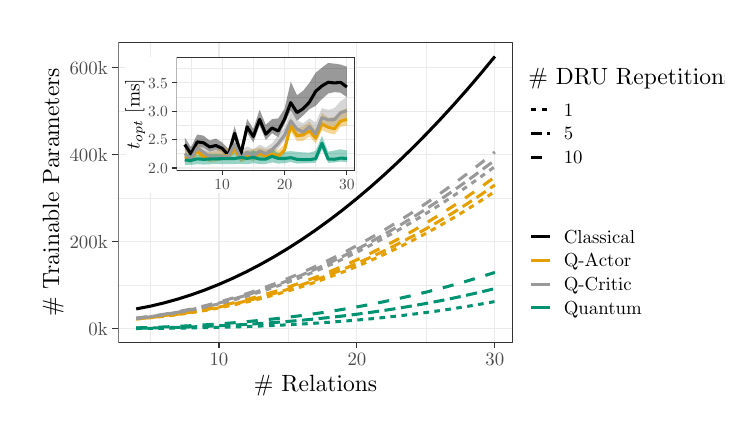
\begin{tikzpicture}[x=1pt,y=1pt]
\definecolor{fillColor}{RGB}{255,255,255}
\path[use as bounding box,fill=fillColor,fill opacity=0.00] (0,0) rectangle (251.96,138.58);
\begin{scope}
\path[clip] (  0.00,  0.00) rectangle (251.96,138.58);
\definecolor{drawColor}{RGB}{255,255,255}
\definecolor{fillColor}{RGB}{255,255,255}

\path[draw=drawColor,line width= 0.6pt,line join=round,line cap=round,fill=fillColor] (  0.00,  0.00) rectangle (251.96,138.58);
\end{scope}
\begin{scope}
\path[clip] (  5.50,  5.50) rectangle (246.46,133.08);
\definecolor{drawColor}{RGB}{255,255,255}
\definecolor{fillColor}{RGB}{255,255,255}

\path[draw=drawColor,line width= 0.4pt,line join=round,line cap=round,fill=fillColor] (  5.50,  5.50) rectangle (246.46,133.08);
\end{scope}
\begin{scope}
\path[clip] ( 32.74, 24.96) rectangle (175.29,133.08);
\definecolor{fillColor}{RGB}{255,255,255}

\path[fill=fillColor] ( 32.74, 24.96) rectangle (175.29,133.08);
\definecolor{drawColor}{gray}{0.92}

\path[draw=drawColor,line width= 0.2pt,line join=round] ( 32.74, 45.55) --
	(175.29, 45.55);

\path[draw=drawColor,line width= 0.2pt,line join=round] ( 32.74, 76.99) --
	(175.29, 76.99);

\path[draw=drawColor,line width= 0.2pt,line join=round] ( 32.74,108.43) --
	(175.29,108.43);

\path[draw=drawColor,line width= 0.2pt,line join=round] ( 44.21, 24.96) --
	( 44.21,133.08);

\path[draw=drawColor,line width= 0.2pt,line join=round] ( 94.05, 24.96) --
	( 94.05,133.08);

\path[draw=drawColor,line width= 0.2pt,line join=round] (143.89, 24.96) --
	(143.89,133.08);

\path[draw=drawColor,line width= 0.4pt,line join=round] ( 32.74, 29.83) --
	(175.29, 29.83);

\path[draw=drawColor,line width= 0.4pt,line join=round] ( 32.74, 61.27) --
	(175.29, 61.27);

\path[draw=drawColor,line width= 0.4pt,line join=round] ( 32.74, 92.71) --
	(175.29, 92.71);

\path[draw=drawColor,line width= 0.4pt,line join=round] ( 32.74,124.15) --
	(175.29,124.15);

\path[draw=drawColor,line width= 0.4pt,line join=round] ( 69.13, 24.96) --
	( 69.13,133.08);

\path[draw=drawColor,line width= 0.4pt,line join=round] (118.97, 24.96) --
	(118.97,133.08);

\path[draw=drawColor,line width= 0.4pt,line join=round] (168.82, 24.96) --
	(168.82,133.08);
\definecolor{drawColor}{RGB}{0,0,0}

\path[draw=drawColor,line width= 1.1pt,line join=round] ( 39.22, 36.95) --
	( 44.21, 37.92) --
	( 49.19, 39.10) --
	( 54.17, 40.48) --
	( 59.16, 42.06) --
	( 64.14, 43.84) --
	( 69.13, 45.83) --
	( 74.11, 48.02) --
	( 79.10, 50.41) --
	( 84.08, 53.01) --
	( 89.07, 55.81) --
	( 94.05, 58.81) --
	( 99.03, 62.01) --
	(104.02, 65.42) --
	(109.00, 69.03) --
	(113.99, 72.84) --
	(118.97, 76.86) --
	(123.96, 81.08) --
	(128.94, 85.50) --
	(133.92, 90.12) --
	(138.91, 94.95) --
	(143.89, 99.98) --
	(148.88,105.21) --
	(153.86,110.64) --
	(158.85,116.28) --
	(163.83,122.12) --
	(168.82,128.17);
\definecolor{drawColor}{RGB}{230,159,0}

\path[draw=drawColor,line width= 1.1pt,dash pattern=on 2pt off 2pt ,line join=round] ( 39.22, 33.31) --
	( 44.21, 33.74) --
	( 49.19, 34.27) --
	( 54.17, 34.88) --
	( 59.16, 35.60) --
	( 64.14, 36.41) --
	( 69.13, 37.32) --
	( 74.11, 38.34) --
	( 79.10, 39.45) --
	( 84.08, 40.67) --
	( 89.07, 42.00) --
	( 94.05, 43.44) --
	( 99.03, 44.99) --
	(104.02, 46.65) --
	(109.00, 48.43) --
	(113.99, 50.32) --
	(118.97, 52.33) --
	(123.96, 54.47) --
	(128.94, 56.72) --
	(133.92, 59.10) --
	(138.91, 61.60) --
	(143.89, 64.24) --
	(148.88, 67.00) --
	(153.86, 69.89) --
	(158.85, 72.92) --
	(163.83, 76.09) --
	(168.82, 79.39);

\path[draw=drawColor,line width= 1.1pt,dash pattern=on 4pt off 2pt ,line join=round] ( 39.22, 33.36) --
	( 44.21, 33.82) --
	( 49.19, 34.37) --
	( 54.17, 35.03) --
	( 59.16, 35.78) --
	( 64.14, 36.64) --
	( 69.13, 37.60) --
	( 74.11, 38.67) --
	( 79.10, 39.84) --
	( 84.08, 41.13) --
	( 89.07, 42.53) --
	( 94.05, 44.04) --
	( 99.03, 45.67) --
	(104.02, 47.42) --
	(109.00, 49.29) --
	(113.99, 51.28) --
	(118.97, 53.39) --
	(123.96, 55.63) --
	(128.94, 57.99) --
	(133.92, 60.49) --
	(138.91, 63.11) --
	(143.89, 65.87) --
	(148.88, 68.77) --
	(153.86, 71.80) --
	(158.85, 74.97) --
	(163.83, 78.27) --
	(168.82, 81.73);

\path[draw=drawColor,line width= 1.1pt,dash pattern=on 4pt off 4pt ,line join=round] ( 39.22, 33.42) --
	( 44.21, 33.91) --
	( 49.19, 34.50) --
	( 54.17, 35.20) --
	( 59.16, 36.01) --
	( 64.14, 36.92) --
	( 69.13, 37.94) --
	( 74.11, 39.08) --
	( 79.10, 40.33) --
	( 84.08, 41.70) --
	( 89.07, 43.19) --
	( 94.05, 44.80) --
	( 99.03, 46.53) --
	(104.02, 48.38) --
	(109.00, 50.36) --
	(113.99, 52.47) --
	(118.97, 54.71) --
	(123.96, 57.08) --
	(128.94, 59.58) --
	(133.92, 62.22) --
	(138.91, 65.00) --
	(143.89, 67.92) --
	(148.88, 70.97) --
	(153.86, 74.17) --
	(158.85, 77.52) --
	(163.83, 81.01) --
	(168.82, 84.65);
\definecolor{drawColor}{gray}{0.60}

\path[draw=drawColor,line width= 1.1pt,dash pattern=on 2pt off 2pt ,line join=round] ( 39.22, 33.51) --
	( 44.21, 34.09) --
	( 49.19, 34.78) --
	( 54.17, 35.60) --
	( 59.16, 36.55) --
	( 64.14, 37.61) --
	( 69.13, 38.80) --
	( 74.11, 40.11) --
	( 79.10, 41.55) --
	( 84.08, 43.11) --
	( 89.07, 44.79) --
	( 94.05, 46.59) --
	( 99.03, 48.52) --
	(104.02, 50.57) --
	(109.00, 52.74) --
	(113.99, 55.03) --
	(118.97, 57.45) --
	(123.96, 59.99) --
	(128.94, 62.66) --
	(133.92, 65.44) --
	(138.91, 68.35) --
	(143.89, 71.39) --
	(148.88, 74.54) --
	(153.86, 77.82) --
	(158.85, 81.22) --
	(163.83, 84.75) --
	(168.82, 88.39);

\path[draw=drawColor,line width= 1.1pt,dash pattern=on 4pt off 2pt ,line join=round] ( 39.22, 33.56) --
	( 44.21, 34.16) --
	( 49.19, 34.89) --
	( 54.17, 35.75) --
	( 59.16, 36.73) --
	( 64.14, 37.84) --
	( 69.13, 39.08) --
	( 74.11, 40.45) --
	( 79.10, 41.94) --
	( 84.08, 43.56) --
	( 89.07, 45.31) --
	( 94.05, 47.19) --
	( 99.03, 49.20) --
	(104.02, 51.34) --
	(109.00, 53.60) --
	(113.99, 55.99) --
	(118.97, 58.51) --
	(123.96, 61.15) --
	(128.94, 63.93) --
	(133.92, 66.83) --
	(138.91, 69.86) --
	(143.89, 73.02) --
	(148.88, 76.31) --
	(153.86, 79.72) --
	(158.85, 83.26) --
	(163.83, 86.94) --
	(168.82, 90.73);

\path[draw=drawColor,line width= 1.1pt,dash pattern=on 4pt off 4pt ,line join=round] ( 39.22, 33.63) --
	( 44.21, 34.26) --
	( 49.19, 35.02) --
	( 54.17, 35.92) --
	( 59.16, 36.95) --
	( 64.14, 38.12) --
	( 69.13, 39.42) --
	( 74.11, 40.86) --
	( 79.10, 42.43) --
	( 84.08, 44.14) --
	( 89.07, 45.98) --
	( 94.05, 47.95) --
	( 99.03, 50.06) --
	(104.02, 52.30) --
	(109.00, 54.67) --
	(113.99, 57.18) --
	(118.97, 59.83) --
	(123.96, 62.61) --
	(128.94, 65.52) --
	(133.92, 68.57) --
	(138.91, 71.75) --
	(143.89, 75.06) --
	(148.88, 78.52) --
	(153.86, 82.10) --
	(158.85, 85.82) --
	(163.83, 89.67) --
	(168.82, 93.66);
\definecolor{drawColor}{RGB}{0,147,113}

\path[draw=drawColor,line width= 1.1pt,dash pattern=on 2pt off 2pt ,line join=round] ( 39.22, 29.88) --
	( 44.21, 29.91) --
	( 49.19, 29.95) --
	( 54.17, 30.01) --
	( 59.16, 30.09) --
	( 64.14, 30.18) --
	( 69.13, 30.29) --
	( 74.11, 30.43) --
	( 79.10, 30.59) --
	( 84.08, 30.77) --
	( 89.07, 30.98) --
	( 94.05, 31.22) --
	( 99.03, 31.49) --
	(104.02, 31.80) --
	(109.00, 32.14) --
	(113.99, 32.51) --
	(118.97, 32.93) --
	(123.96, 33.38) --
	(128.94, 33.88) --
	(133.92, 34.42) --
	(138.91, 35.01) --
	(143.89, 35.65) --
	(148.88, 36.33) --
	(153.86, 37.07) --
	(158.85, 37.86) --
	(163.83, 38.71) --
	(168.82, 39.62);

\path[draw=drawColor,line width= 1.1pt,dash pattern=on 4pt off 2pt ,line join=round] ( 39.22, 29.98) --
	( 44.21, 30.06) --
	( 49.19, 30.17) --
	( 54.17, 30.29) --
	( 59.16, 30.45) --
	( 64.14, 30.63) --
	( 69.13, 30.85) --
	( 74.11, 31.09) --
	( 79.10, 31.37) --
	( 84.08, 31.69) --
	( 89.07, 32.04) --
	( 94.05, 32.43) --
	( 99.03, 32.86) --
	(104.02, 33.34) --
	(109.00, 33.86) --
	(113.99, 34.42) --
	(118.97, 35.04) --
	(123.96, 35.71) --
	(128.94, 36.43) --
	(133.92, 37.20) --
	(138.91, 38.03) --
	(143.89, 38.92) --
	(148.88, 39.86) --
	(153.86, 40.87) --
	(158.85, 41.95) --
	(163.83, 43.09) --
	(168.82, 44.29);

\path[draw=drawColor,line width= 1.1pt,dash pattern=on 4pt off 4pt ,line join=round] ( 39.22, 30.10) --
	( 44.21, 30.25) --
	( 49.19, 30.43) --
	( 54.17, 30.65) --
	( 59.16, 30.90) --
	( 64.14, 31.20) --
	( 69.13, 31.54) --
	( 74.11, 31.92) --
	( 79.10, 32.35) --
	( 84.08, 32.83) --
	( 89.07, 33.36) --
	( 94.05, 33.94) --
	( 99.03, 34.57) --
	(104.02, 35.26) --
	(109.00, 36.01) --
	(113.99, 36.81) --
	(118.97, 37.68) --
	(123.96, 38.61) --
	(128.94, 39.61) --
	(133.92, 40.67) --
	(138.91, 41.80) --
	(143.89, 43.00) --
	(148.88, 44.28) --
	(153.86, 45.63) --
	(158.85, 47.05) --
	(163.83, 48.56) --
	(168.82, 50.14);
\definecolor{drawColor}{gray}{0.20}

\path[draw=drawColor,line width= 0.4pt,line join=round,line cap=round] ( 32.74, 24.96) rectangle (175.29,133.08);
\end{scope}
\begin{scope}
\path[clip] (  0.00,  0.00) rectangle (251.96,138.58);
\definecolor{drawColor}{gray}{0.30}

\node[text=drawColor,anchor=base east,inner sep=0pt, outer sep=0pt, scale=  0.68] at ( 28.92, 27.49) {0k};

\node[text=drawColor,anchor=base east,inner sep=0pt, outer sep=0pt, scale=  0.68] at ( 28.92, 58.93) {200k};

\node[text=drawColor,anchor=base east,inner sep=0pt, outer sep=0pt, scale=  0.68] at ( 28.92, 90.37) {400k};

\node[text=drawColor,anchor=base east,inner sep=0pt, outer sep=0pt, scale=  0.68] at ( 28.92,121.81) {600k};
\end{scope}
\begin{scope}
\path[clip] (  0.00,  0.00) rectangle (251.96,138.58);
\definecolor{drawColor}{gray}{0.20}

\path[draw=drawColor,line width= 0.4pt,line join=round] ( 30.62, 29.83) --
	( 32.74, 29.83);

\path[draw=drawColor,line width= 0.4pt,line join=round] ( 30.62, 61.27) --
	( 32.74, 61.27);

\path[draw=drawColor,line width= 0.4pt,line join=round] ( 30.62, 92.71) --
	( 32.74, 92.71);

\path[draw=drawColor,line width= 0.4pt,line join=round] ( 30.62,124.15) --
	( 32.74,124.15);
\end{scope}
\begin{scope}
\path[clip] (  0.00,  0.00) rectangle (251.96,138.58);
\definecolor{drawColor}{gray}{0.20}

\path[draw=drawColor,line width= 0.4pt,line join=round] ( 69.13, 22.84) --
	( 69.13, 24.96);

\path[draw=drawColor,line width= 0.4pt,line join=round] (118.97, 22.84) --
	(118.97, 24.96);

\path[draw=drawColor,line width= 0.4pt,line join=round] (168.82, 22.84) --
	(168.82, 24.96);
\end{scope}
\begin{scope}
\path[clip] (  0.00,  0.00) rectangle (251.96,138.58);
\definecolor{drawColor}{gray}{0.30}

\node[text=drawColor,anchor=base,inner sep=0pt, outer sep=0pt, scale=  0.68] at ( 69.13, 16.45) {10};

\node[text=drawColor,anchor=base,inner sep=0pt, outer sep=0pt, scale=  0.68] at (118.97, 16.45) {20};

\node[text=drawColor,anchor=base,inner sep=0pt, outer sep=0pt, scale=  0.68] at (168.82, 16.45) {30};
\end{scope}
\begin{scope}
\path[clip] (  0.00,  0.00) rectangle (251.96,138.58);
\definecolor{drawColor}{RGB}{0,0,0}

\node[text=drawColor,anchor=base,inner sep=0pt, outer sep=0pt, scale=  0.85] at (104.02,  7.15) {\# Relations};
\end{scope}
\begin{scope}
\path[clip] (  0.00,  0.00) rectangle (251.96,138.58);
\definecolor{drawColor}{RGB}{0,0,0}

\node[text=drawColor,rotate= 90.00,anchor=base,inner sep=0pt, outer sep=0pt, scale=  0.85] at ( 11.35, 79.02) {\# Trainable Parameters};
\end{scope}
\begin{scope}
\path[clip] (  0.00,  0.00) rectangle (251.96,138.58);
\definecolor{fillColor}{RGB}{255,255,255}

\path[fill=fillColor] (183.79, 87.54) rectangle (246.46,124.90);
\end{scope}
\begin{scope}
\path[clip] (  0.00,  0.00) rectangle (251.96,138.58);
\definecolor{drawColor}{RGB}{0,0,0}

\node[text=drawColor,anchor=base west,inner sep=0pt, outer sep=0pt, scale=  0.85] at (180.95,118.22) {\# DRU Repetitions};
\end{scope}
\begin{scope}
\path[clip] (  0.00,  0.00) rectangle (251.96,138.58);
\definecolor{fillColor}{RGB}{255,255,255}

\path[fill=fillColor] (180.95,104.61) rectangle (189.49,113.15);
\end{scope}
\begin{scope}
\path[clip] (  0.00,  0.00) rectangle (251.96,138.58);
\definecolor{drawColor}{RGB}{0,0,0}

\path[draw=drawColor,line width= 1.1pt,dash pattern=on 2pt off 2pt ,line join=round] (181.80,108.88) -- (188.63,108.88);
\end{scope}
\begin{scope}
\path[clip] (  0.00,  0.00) rectangle (251.96,138.58);
\definecolor{fillColor}{RGB}{255,255,255}

\path[fill=fillColor] (180.95, 96.07) rectangle (189.49,104.61);
\end{scope}
\begin{scope}
\path[clip] (  0.00,  0.00) rectangle (251.96,138.58);
\definecolor{drawColor}{RGB}{0,0,0}

\path[draw=drawColor,line width= 1.1pt,dash pattern=on 4pt off 2pt ,line join=round] (181.80,100.34) -- (188.63,100.34);
\end{scope}
\begin{scope}
\path[clip] (  0.00,  0.00) rectangle (251.96,138.58);
\definecolor{fillColor}{RGB}{255,255,255}

\path[fill=fillColor] (180.95, 87.54) rectangle (189.49, 96.07);
\end{scope}
\begin{scope}
\path[clip] (  0.00,  0.00) rectangle (251.96,138.58);
\definecolor{drawColor}{RGB}{0,0,0}

\path[draw=drawColor,line width= 1.1pt,dash pattern=on 4pt off 4pt ,line join=round] (181.80, 91.81) -- (188.63, 91.81);
\end{scope}
\begin{scope}
\path[clip] (  0.00,  0.00) rectangle (251.96,138.58);
\definecolor{drawColor}{RGB}{0,0,0}

\node[text=drawColor,anchor=base west,inner sep=0pt, outer sep=0pt, scale=  0.68] at (193.74,106.54) {1};
\end{scope}
\begin{scope}
\path[clip] (  0.00,  0.00) rectangle (251.96,138.58);
\definecolor{drawColor}{RGB}{0,0,0}

\node[text=drawColor,anchor=base west,inner sep=0pt, outer sep=0pt, scale=  0.68] at (193.74, 98.00) {5};
\end{scope}
\begin{scope}
\path[clip] (  0.00,  0.00) rectangle (251.96,138.58);
\definecolor{drawColor}{RGB}{0,0,0}

\node[text=drawColor,anchor=base west,inner sep=0pt, outer sep=0pt, scale=  0.68] at (193.74, 89.47) {10};
\end{scope}
\begin{scope}
\path[clip] (  0.00,  0.00) rectangle (251.96,138.58);
\definecolor{fillColor}{RGB}{255,255,255}

\path[fill=fillColor] (183.79, 33.14) rectangle (213.34, 79.04);
\end{scope}
\begin{scope}
\path[clip] (  0.00,  0.00) rectangle (251.96,138.58);
\definecolor{fillColor}{RGB}{255,255,255}

\path[fill=fillColor] (180.95, 58.75) rectangle (189.49, 67.28);
\end{scope}
\begin{scope}
\path[clip] (  0.00,  0.00) rectangle (251.96,138.58);
\definecolor{drawColor}{RGB}{0,0,0}

\path[draw=drawColor,line width= 1.1pt,line join=round] (181.80, 63.01) -- (188.63, 63.01);
\end{scope}
\begin{scope}
\path[clip] (  0.00,  0.00) rectangle (251.96,138.58);
\definecolor{fillColor}{RGB}{255,255,255}

\path[fill=fillColor] (180.95, 50.21) rectangle (189.49, 58.75);
\end{scope}
\begin{scope}
\path[clip] (  0.00,  0.00) rectangle (251.96,138.58);
\definecolor{drawColor}{RGB}{230,159,0}

\path[draw=drawColor,line width= 1.1pt,line join=round] (181.80, 54.48) -- (188.63, 54.48);
\end{scope}
\begin{scope}
\path[clip] (  0.00,  0.00) rectangle (251.96,138.58);
\definecolor{fillColor}{RGB}{255,255,255}

\path[fill=fillColor] (180.95, 41.67) rectangle (189.49, 50.21);
\end{scope}
\begin{scope}
\path[clip] (  0.00,  0.00) rectangle (251.96,138.58);
\definecolor{drawColor}{gray}{0.60}

\path[draw=drawColor,line width= 1.1pt,line join=round] (181.80, 45.94) -- (188.63, 45.94);
\end{scope}
\begin{scope}
\path[clip] (  0.00,  0.00) rectangle (251.96,138.58);
\definecolor{fillColor}{RGB}{255,255,255}

\path[fill=fillColor] (180.95, 33.14) rectangle (189.49, 41.67);
\end{scope}
\begin{scope}
\path[clip] (  0.00,  0.00) rectangle (251.96,138.58);
\definecolor{drawColor}{RGB}{0,147,113}

\path[draw=drawColor,line width= 1.1pt,line join=round] (181.80, 37.41) -- (188.63, 37.41);
\end{scope}
\begin{scope}
\path[clip] (  0.00,  0.00) rectangle (251.96,138.58);
\definecolor{drawColor}{RGB}{0,0,0}

\node[text=drawColor,anchor=base west,inner sep=0pt, outer sep=0pt, scale=  0.68] at (193.74, 60.67) {Classical};
\end{scope}
\begin{scope}
\path[clip] (  0.00,  0.00) rectangle (251.96,138.58);
\definecolor{drawColor}{RGB}{0,0,0}

\node[text=drawColor,anchor=base west,inner sep=0pt, outer sep=0pt, scale=  0.68] at (193.74, 52.14) {Q-Actor};
\end{scope}
\begin{scope}
\path[clip] (  0.00,  0.00) rectangle (251.96,138.58);
\definecolor{drawColor}{RGB}{0,0,0}

\node[text=drawColor,anchor=base west,inner sep=0pt, outer sep=0pt, scale=  0.68] at (193.74, 43.60) {Q-Critic};
\end{scope}
\begin{scope}
\path[clip] (  0.00,  0.00) rectangle (251.96,138.58);
\definecolor{drawColor}{RGB}{0,0,0}

\node[text=drawColor,anchor=base west,inner sep=0pt, outer sep=0pt, scale=  0.68] at (193.74, 35.07) {Quantum};
\end{scope}
\begin{scope}
\path[clip] ( 35.59, 79.02) rectangle (118.27,127.67);
\definecolor{drawColor}{RGB}{255,255,255}
\definecolor{fillColor}{RGB}{255,255,255}

\path[draw=drawColor,line width= 0.4pt,line join=round,line cap=round,fill=fillColor] ( 35.59, 79.02) rectangle (118.27,127.67);
\end{scope}
\begin{scope}
\path[clip] ( 53.83, 87.12) rectangle (118.27,127.67);

\path[] ( 53.83, 87.12) rectangle (118.27,127.67);
\definecolor{drawColor}{gray}{0.92}

\path[draw=drawColor,line width= 0.2pt,line join=round] ( 53.83, 93.02) --
	(118.27, 93.02);

\path[draw=drawColor,line width= 0.2pt,line join=round] ( 53.83,103.28) --
	(118.27,103.28);

\path[draw=drawColor,line width= 0.2pt,line join=round] ( 53.83,113.55) --
	(118.27,113.55);

\path[draw=drawColor,line width= 0.2pt,line join=round] ( 53.83,123.82) --
	(118.27,123.82);

\path[draw=drawColor,line width= 0.2pt,line join=round] ( 59.01, 87.12) --
	( 59.01,127.67);

\path[draw=drawColor,line width= 0.2pt,line join=round] ( 81.54, 87.12) --
	( 81.54,127.67);

\path[draw=drawColor,line width= 0.2pt,line join=round] (104.08, 87.12) --
	(104.08,127.67);

\path[draw=drawColor,line width= 0.4pt,line join=round] ( 53.83, 87.88) --
	(118.27, 87.88);

\path[draw=drawColor,line width= 0.4pt,line join=round] ( 53.83, 98.15) --
	(118.27, 98.15);

\path[draw=drawColor,line width= 0.4pt,line join=round] ( 53.83,108.42) --
	(118.27,108.42);

\path[draw=drawColor,line width= 0.4pt,line join=round] ( 53.83,118.69) --
	(118.27,118.69);

\path[draw=drawColor,line width= 0.4pt,line join=round] ( 70.28, 87.12) --
	( 70.28,127.67);

\path[draw=drawColor,line width= 0.4pt,line join=round] ( 92.81, 87.12) --
	( 92.81,127.67);

\path[draw=drawColor,line width= 0.4pt,line join=round] (115.34, 87.12) --
	(115.34,127.67);
\definecolor{fillColor}{RGB}{0,0,0}

\path[fill=fillColor,fill opacity=0.40] ( 56.76, 98.94) --
	( 59.01, 95.38) --
	( 61.26, 99.97) --
	( 63.52, 99.56) --
	( 65.77, 97.78) --
	( 68.02, 98.52) --
	( 70.28, 97.12) --
	( 72.53, 94.75) --
	( 74.78,102.99) --
	( 77.04, 95.14) --
	( 79.29,105.60) --
	( 81.54,102.02) --
	( 83.80,108.92) --
	( 86.05,103.49) --
	( 88.30,105.53) --
	( 90.56,105.83) --
	( 92.81,109.22) --
	( 95.06,119.05) --
	( 97.32,114.19) --
	( 99.57,115.84) --
	(101.82,118.66) --
	(104.08,122.30) --
	(106.33,124.13) --
	(108.58,125.83) --
	(110.84,125.59) --
	(113.09,125.24) --
	(115.34,124.49) --
	(115.34,113.46) --
	(113.09,115.08) --
	(110.84,115.29) --
	(108.58,114.79) --
	(106.33,112.79) --
	(104.08,110.36) --
	(101.82,109.14) --
	( 99.57,106.90) --
	( 97.32,104.88) --
	( 95.06,108.69) --
	( 92.81,103.73) --
	( 90.56, 99.00) --
	( 88.30,100.45) --
	( 86.05, 97.93) --
	( 83.80,103.23) --
	( 81.54, 97.13) --
	( 79.29,100.67) --
	( 77.04, 91.72) --
	( 74.78, 98.66) --
	( 72.53, 91.23) --
	( 70.28, 93.71) --
	( 68.02, 94.43) --
	( 65.77, 93.78) --
	( 63.52, 95.28) --
	( 61.26, 95.54) --
	( 59.01, 91.57) --
	( 56.76, 94.67) --
	cycle;

\path[] ( 56.76, 98.94) --
	( 59.01, 95.38) --
	( 61.26, 99.97) --
	( 63.52, 99.56) --
	( 65.77, 97.78) --
	( 68.02, 98.52) --
	( 70.28, 97.12) --
	( 72.53, 94.75) --
	( 74.78,102.99) --
	( 77.04, 95.14) --
	( 79.29,105.60) --
	( 81.54,102.02) --
	( 83.80,108.92) --
	( 86.05,103.49) --
	( 88.30,105.53) --
	( 90.56,105.83) --
	( 92.81,109.22) --
	( 95.06,119.05) --
	( 97.32,114.19) --
	( 99.57,115.84) --
	(101.82,118.66) --
	(104.08,122.30) --
	(106.33,124.13) --
	(108.58,125.83) --
	(110.84,125.59) --
	(113.09,125.24) --
	(115.34,124.49);

\path[] (115.34,113.46) --
	(113.09,115.08) --
	(110.84,115.29) --
	(108.58,114.79) --
	(106.33,112.79) --
	(104.08,110.36) --
	(101.82,109.14) --
	( 99.57,106.90) --
	( 97.32,104.88) --
	( 95.06,108.69) --
	( 92.81,103.73) --
	( 90.56, 99.00) --
	( 88.30,100.45) --
	( 86.05, 97.93) --
	( 83.80,103.23) --
	( 81.54, 97.13) --
	( 79.29,100.67) --
	( 77.04, 91.72) --
	( 74.78, 98.66) --
	( 72.53, 91.23) --
	( 70.28, 93.71) --
	( 68.02, 94.43) --
	( 65.77, 93.78) --
	( 63.52, 95.28) --
	( 61.26, 95.54) --
	( 59.01, 91.57) --
	( 56.76, 94.67);
\definecolor{fillColor}{RGB}{230,159,0}

\path[fill=fillColor,fill opacity=0.40] ( 56.76, 94.53) --
	( 59.01, 93.48) --
	( 61.26, 96.64) --
	( 63.52, 94.10) --
	( 65.77, 93.62) --
	( 68.02, 94.00) --
	( 70.28, 95.07) --
	( 72.53, 95.05) --
	( 74.78, 96.83) --
	( 77.04, 93.77) --
	( 79.29, 94.16) --
	( 81.54, 94.70) --
	( 83.80, 95.23) --
	( 86.05, 94.63) --
	( 88.30, 95.11) --
	( 90.56, 94.37) --
	( 92.81, 96.57) --
	( 95.06,105.99) --
	( 97.32,102.29) --
	( 99.57,102.92) --
	(101.82,104.57) --
	(104.08,101.64) --
	(106.33,107.82) --
	(108.58,106.05) --
	(110.84,106.28) --
	(113.09,108.55) --
	(115.34,109.45) --
	(115.34,103.18) --
	(113.09,102.76) --
	(110.84, 99.92) --
	(108.58,100.54) --
	(106.33,101.51) --
	(104.08, 96.70) --
	(101.82, 99.35) --
	( 99.57, 97.65) --
	( 97.32, 97.55) --
	( 95.06,101.03) --
	( 92.81, 93.02) --
	( 90.56, 91.01) --
	( 88.30, 91.69) --
	( 86.05, 90.80) --
	( 83.80, 92.03) --
	( 81.54, 90.42) --
	( 79.29, 90.91) --
	( 77.04, 89.88) --
	( 74.78, 93.06) --
	( 72.53, 90.66) --
	( 70.28, 90.81) --
	( 68.02, 90.22) --
	( 65.77, 90.03) --
	( 63.52, 90.63) --
	( 61.26, 92.36) --
	( 59.01, 89.68) --
	( 56.76, 90.42) --
	cycle;

\path[] ( 56.76, 94.53) --
	( 59.01, 93.48) --
	( 61.26, 96.64) --
	( 63.52, 94.10) --
	( 65.77, 93.62) --
	( 68.02, 94.00) --
	( 70.28, 95.07) --
	( 72.53, 95.05) --
	( 74.78, 96.83) --
	( 77.04, 93.77) --
	( 79.29, 94.16) --
	( 81.54, 94.70) --
	( 83.80, 95.23) --
	( 86.05, 94.63) --
	( 88.30, 95.11) --
	( 90.56, 94.37) --
	( 92.81, 96.57) --
	( 95.06,105.99) --
	( 97.32,102.29) --
	( 99.57,102.92) --
	(101.82,104.57) --
	(104.08,101.64) --
	(106.33,107.82) --
	(108.58,106.05) --
	(110.84,106.28) --
	(113.09,108.55) --
	(115.34,109.45);

\path[] (115.34,103.18) --
	(113.09,102.76) --
	(110.84, 99.92) --
	(108.58,100.54) --
	(106.33,101.51) --
	(104.08, 96.70) --
	(101.82, 99.35) --
	( 99.57, 97.65) --
	( 97.32, 97.55) --
	( 95.06,101.03) --
	( 92.81, 93.02) --
	( 90.56, 91.01) --
	( 88.30, 91.69) --
	( 86.05, 90.80) --
	( 83.80, 92.03) --
	( 81.54, 90.42) --
	( 79.29, 90.91) --
	( 77.04, 89.88) --
	( 74.78, 93.06) --
	( 72.53, 90.66) --
	( 70.28, 90.81) --
	( 68.02, 90.22) --
	( 65.77, 90.03) --
	( 63.52, 90.63) --
	( 61.26, 92.36) --
	( 59.01, 89.68) --
	( 56.76, 90.42);
\definecolor{fillColor}{RGB}{153,153,153}

\path[fill=fillColor,fill opacity=0.40] ( 56.76, 95.63) --
	( 59.01, 93.71) --
	( 61.26, 97.71) --
	( 63.52, 95.95) --
	( 65.77, 94.49) --
	( 68.02, 94.33) --
	( 70.28, 94.25) --
	( 72.53, 95.25) --
	( 74.78, 99.00) --
	( 77.04, 94.37) --
	( 79.29, 95.66) --
	( 81.54, 94.61) --
	( 83.80, 96.28) --
	( 86.05, 95.26) --
	( 88.30, 96.81) --
	( 90.56, 99.80) --
	( 92.81,102.46) --
	( 95.06,108.26) --
	( 97.32,105.03) --
	( 99.57,104.05) --
	(101.82,105.84) --
	(104.08,104.24) --
	(106.33,109.52) --
	(108.58,108.88) --
	(110.84,109.51) --
	(113.09,112.06) --
	(115.34,113.48) --
	(115.34,106.15) --
	(113.09,105.46) --
	(110.84,103.12) --
	(108.58,103.17) --
	(106.33,104.06) --
	(104.08, 98.14) --
	(101.82,101.13) --
	( 99.57, 99.01) --
	( 97.32, 99.76) --
	( 95.06,102.80) --
	( 92.81, 97.91) --
	( 90.56, 94.86) --
	( 88.30, 93.16) --
	( 86.05, 91.68) --
	( 83.80, 93.01) --
	( 81.54, 90.60) --
	( 79.29, 92.45) --
	( 77.04, 90.15) --
	( 74.78, 94.79) --
	( 72.53, 90.81) --
	( 70.28, 90.74) --
	( 68.02, 90.56) --
	( 65.77, 90.66) --
	( 63.52, 91.88) --
	( 61.26, 93.24) --
	( 59.01, 89.82) --
	( 56.76, 91.60) --
	cycle;

\path[] ( 56.76, 95.63) --
	( 59.01, 93.71) --
	( 61.26, 97.71) --
	( 63.52, 95.95) --
	( 65.77, 94.49) --
	( 68.02, 94.33) --
	( 70.28, 94.25) --
	( 72.53, 95.25) --
	( 74.78, 99.00) --
	( 77.04, 94.37) --
	( 79.29, 95.66) --
	( 81.54, 94.61) --
	( 83.80, 96.28) --
	( 86.05, 95.26) --
	( 88.30, 96.81) --
	( 90.56, 99.80) --
	( 92.81,102.46) --
	( 95.06,108.26) --
	( 97.32,105.03) --
	( 99.57,104.05) --
	(101.82,105.84) --
	(104.08,104.24) --
	(106.33,109.52) --
	(108.58,108.88) --
	(110.84,109.51) --
	(113.09,112.06) --
	(115.34,113.48);

\path[] (115.34,106.15) --
	(113.09,105.46) --
	(110.84,103.12) --
	(108.58,103.17) --
	(106.33,104.06) --
	(104.08, 98.14) --
	(101.82,101.13) --
	( 99.57, 99.01) --
	( 97.32, 99.76) --
	( 95.06,102.80) --
	( 92.81, 97.91) --
	( 90.56, 94.86) --
	( 88.30, 93.16) --
	( 86.05, 91.68) --
	( 83.80, 93.01) --
	( 81.54, 90.60) --
	( 79.29, 92.45) --
	( 77.04, 90.15) --
	( 74.78, 94.79) --
	( 72.53, 90.81) --
	( 70.28, 90.74) --
	( 68.02, 90.56) --
	( 65.77, 90.66) --
	( 63.52, 91.88) --
	( 61.26, 93.24) --
	( 59.01, 89.82) --
	( 56.76, 91.60);
\definecolor{fillColor}{RGB}{0,147,113}

\path[fill=fillColor,fill opacity=0.40] ( 56.76, 92.81) --
	( 59.01, 92.97) --
	( 61.26, 92.73) --
	( 63.52, 92.77) --
	( 65.77, 92.95) --
	( 68.02, 92.85) --
	( 70.28, 92.88) --
	( 72.53, 92.90) --
	( 74.78, 93.43) --
	( 77.04, 93.55) --
	( 79.29, 93.35) --
	( 81.54, 94.17) --
	( 83.80, 93.38) --
	( 86.05, 93.32) --
	( 88.30, 94.59) --
	( 90.56, 93.34) --
	( 92.81, 93.77) --
	( 95.06, 93.96) --
	( 97.32, 93.73) --
	( 99.57, 93.51) --
	(101.82, 93.42) --
	(104.08, 94.06) --
	(106.33, 99.46) --
	(108.58, 93.74) --
	(110.84, 94.19) --
	(113.09, 94.64) --
	(115.34, 94.15) --
	(115.34, 90.00) --
	(113.09, 90.19) --
	(110.84, 89.86) --
	(108.58, 89.73) --
	(106.33, 94.59) --
	(104.08, 89.81) --
	(101.82, 89.63) --
	( 99.57, 89.54) --
	( 97.32, 89.48) --
	( 95.06, 90.03) --
	( 92.81, 89.62) --
	( 90.56, 89.44) --
	( 88.30, 89.92) --
	( 86.05, 89.33) --
	( 83.80, 89.26) --
	( 81.54, 89.62) --
	( 79.29, 89.24) --
	( 77.04, 89.36) --
	( 74.78, 89.29) --
	( 72.53, 89.27) --
	( 70.28, 89.26) --
	( 68.02, 89.36) --
	( 65.77, 89.20) --
	( 63.52, 89.11) --
	( 61.26, 89.27) --
	( 59.01, 88.96) --
	( 56.76, 89.00) --
	cycle;

\path[] ( 56.76, 92.81) --
	( 59.01, 92.97) --
	( 61.26, 92.73) --
	( 63.52, 92.77) --
	( 65.77, 92.95) --
	( 68.02, 92.85) --
	( 70.28, 92.88) --
	( 72.53, 92.90) --
	( 74.78, 93.43) --
	( 77.04, 93.55) --
	( 79.29, 93.35) --
	( 81.54, 94.17) --
	( 83.80, 93.38) --
	( 86.05, 93.32) --
	( 88.30, 94.59) --
	( 90.56, 93.34) --
	( 92.81, 93.77) --
	( 95.06, 93.96) --
	( 97.32, 93.73) --
	( 99.57, 93.51) --
	(101.82, 93.42) --
	(104.08, 94.06) --
	(106.33, 99.46) --
	(108.58, 93.74) --
	(110.84, 94.19) --
	(113.09, 94.64) --
	(115.34, 94.15);

\path[] (115.34, 90.00) --
	(113.09, 90.19) --
	(110.84, 89.86) --
	(108.58, 89.73) --
	(106.33, 94.59) --
	(104.08, 89.81) --
	(101.82, 89.63) --
	( 99.57, 89.54) --
	( 97.32, 89.48) --
	( 95.06, 90.03) --
	( 92.81, 89.62) --
	( 90.56, 89.44) --
	( 88.30, 89.92) --
	( 86.05, 89.33) --
	( 83.80, 89.26) --
	( 81.54, 89.62) --
	( 79.29, 89.24) --
	( 77.04, 89.36) --
	( 74.78, 89.29) --
	( 72.53, 89.27) --
	( 70.28, 89.26) --
	( 68.02, 89.36) --
	( 65.77, 89.20) --
	( 63.52, 89.11) --
	( 61.26, 89.27) --
	( 59.01, 88.96) --
	( 56.76, 89.00);
\definecolor{drawColor}{RGB}{0,0,0}

\path[draw=drawColor,line width= 1.1pt,line join=round] ( 56.76, 96.36) --
	( 59.01, 92.93) --
	( 61.26, 97.31) --
	( 63.52, 97.00) --
	( 65.77, 95.47) --
	( 68.02, 95.99) --
	( 70.28, 94.97) --
	( 72.53, 92.48) --
	( 74.78,100.42) --
	( 77.04, 92.93) --
	( 79.29,102.74) --
	( 81.54, 99.25) --
	( 83.80,105.45) --
	( 86.05,100.08) --
	( 88.30,102.32) --
	( 90.56,101.25) --
	( 92.81,105.50) --
	( 95.06,111.49) --
	( 97.32,107.91) --
	( 99.57,109.33) --
	(101.82,111.68) --
	(104.08,115.60) --
	(106.33,117.53) --
	(108.58,118.86) --
	(110.84,118.60) --
	(113.09,118.83) --
	(115.34,117.12);
\definecolor{drawColor}{RGB}{230,159,0}

\path[draw=drawColor,line width= 1.1pt,line join=round] ( 56.76, 92.00) --
	( 59.01, 91.25) --
	( 61.26, 94.04) --
	( 63.52, 91.92) --
	( 65.77, 91.28) --
	( 68.02, 91.50) --
	( 70.28, 92.18) --
	( 72.53, 92.38) --
	( 74.78, 94.50) --
	( 77.04, 91.12) --
	( 79.29, 91.99) --
	( 81.54, 91.86) --
	( 83.80, 93.15) --
	( 86.05, 92.13) --
	( 88.30, 92.90) --
	( 90.56, 92.17) --
	( 92.81, 94.37) --
	( 95.06,103.17) --
	( 97.32, 99.47) --
	( 99.57, 99.92) --
	(101.82,101.30) --
	(104.08, 98.62) --
	(106.33,103.75) --
	(108.58,102.60) --
	(110.84,102.05) --
	(113.09,104.78) --
	(115.34,105.46);
\definecolor{drawColor}{gray}{0.60}

\path[draw=drawColor,line width= 1.1pt,line join=round] ( 56.76, 93.09) --
	( 59.01, 91.14) --
	( 61.26, 95.17) --
	( 63.52, 93.57) --
	( 65.77, 91.93) --
	( 68.02, 91.74) --
	( 70.28, 92.01) --
	( 72.53, 92.14) --
	( 74.78, 96.42) --
	( 77.04, 91.32) --
	( 79.29, 93.64) --
	( 81.54, 92.05) --
	( 83.80, 94.04) --
	( 86.05, 93.02) --
	( 88.30, 94.51) --
	( 90.56, 96.77) --
	( 92.81, 99.69) --
	( 95.06,104.90) --
	( 97.32,101.93) --
	( 99.57,100.88) --
	(101.82,102.84) --
	(104.08,100.12) --
	(106.33,106.08) --
	(108.58,105.28) --
	(110.84,105.32) --
	(113.09,107.88) --
	(115.34,108.60);
\definecolor{drawColor}{RGB}{0,147,113}

\path[draw=drawColor,line width= 1.1pt,line join=round] ( 56.76, 90.73) --
	( 59.01, 90.62) --
	( 61.26, 91.18) --
	( 63.52, 91.00) --
	( 65.77, 91.12) --
	( 68.02, 91.19) --
	( 70.28, 91.23) --
	( 72.53, 91.29) --
	( 74.78, 91.29) --
	( 77.04, 91.66) --
	( 79.29, 91.34) --
	( 81.54, 91.71) --
	( 83.80, 91.12) --
	( 86.05, 91.09) --
	( 88.30, 92.10) --
	( 90.56, 91.32) --
	( 92.81, 91.30) --
	( 95.06, 91.61) --
	( 97.32, 91.01) --
	( 99.57, 90.88) --
	(101.82, 90.87) --
	(104.08, 91.25) --
	(106.33, 96.85) --
	(108.58, 91.10) --
	(110.84, 91.03) --
	(113.09, 91.42) --
	(115.34, 91.36);
\definecolor{drawColor}{gray}{0.20}

\path[draw=drawColor,line width= 0.4pt,line join=round,line cap=round] ( 53.83, 87.12) rectangle (118.27,127.67);
\end{scope}
\begin{scope}
\path[clip] (  0.00,  0.00) rectangle (251.96,138.58);
\definecolor{drawColor}{gray}{0.30}

\node[text=drawColor,anchor=base east,inner sep=0pt, outer sep=0pt, scale=  0.56] at ( 50.68, 85.96) {2.0};

\node[text=drawColor,anchor=base east,inner sep=0pt, outer sep=0pt, scale=  0.56] at ( 50.68, 96.22) {2.5};

\node[text=drawColor,anchor=base east,inner sep=0pt, outer sep=0pt, scale=  0.56] at ( 50.68,106.49) {3.0};

\node[text=drawColor,anchor=base east,inner sep=0pt, outer sep=0pt, scale=  0.56] at ( 50.68,116.76) {3.5};
\end{scope}
\begin{scope}
\path[clip] (  0.00,  0.00) rectangle (251.96,138.58);
\definecolor{drawColor}{gray}{0.20}

\path[draw=drawColor,line width= 0.4pt,line join=round] ( 52.08, 87.88) --
	( 53.83, 87.88);

\path[draw=drawColor,line width= 0.4pt,line join=round] ( 52.08, 98.15) --
	( 53.83, 98.15);

\path[draw=drawColor,line width= 0.4pt,line join=round] ( 52.08,108.42) --
	( 53.83,108.42);

\path[draw=drawColor,line width= 0.4pt,line join=round] ( 52.08,118.69) --
	( 53.83,118.69);
\end{scope}
\begin{scope}
\path[clip] (  0.00,  0.00) rectangle (251.96,138.58);
\definecolor{drawColor}{gray}{0.20}

\path[draw=drawColor,line width= 0.4pt,line join=round] ( 70.28, 85.37) --
	( 70.28, 87.12);

\path[draw=drawColor,line width= 0.4pt,line join=round] ( 92.81, 85.37) --
	( 92.81, 87.12);

\path[draw=drawColor,line width= 0.4pt,line join=round] (115.34, 85.37) --
	(115.34, 87.12);
\end{scope}
\begin{scope}
\path[clip] (  0.00,  0.00) rectangle (251.96,138.58);
\definecolor{drawColor}{gray}{0.30}

\node[text=drawColor,anchor=base,inner sep=0pt, outer sep=0pt, scale=  0.56] at ( 70.28, 80.11) {10};

\node[text=drawColor,anchor=base,inner sep=0pt, outer sep=0pt, scale=  0.56] at ( 92.81, 80.11) {20};

\node[text=drawColor,anchor=base,inner sep=0pt, outer sep=0pt, scale=  0.56] at (115.34, 80.11) {30};
\end{scope}
\begin{scope}
\path[clip] (  0.00,  0.00) rectangle (251.96,138.58);
\definecolor{drawColor}{RGB}{0,0,0}

\node[text=drawColor,rotate= 90.00,anchor=base,inner sep=0pt, outer sep=0pt, scale=  0.70] at ( 40.41,107.40) {$t_\text{opt}$ [ms]};
\end{scope}
\end{tikzpicture}
